%
% $RCSfile: structure_by_hierarchy.tex,v $
%
% Copyright (C) 2002-2008. Christian Heller.
%
% Permission is granted to copy, distribute and/or modify this document
% under the terms of the GNU Free Documentation License, Version 1.1 or
% any later version published by the Free Software Foundation; with no
% Invariant Sections, with no Front-Cover Texts and with no Back-Cover
% Texts. A copy of the license is included in the section entitled
% "GNU Free Documentation License".
%
% http://www.cybop.net
% - Cybernetics Oriented Programming -
%
% http://www.resmedicinae.org
% - Information in Medicine -
%
% Version: $Revision: 1.1 $ $Date: 2008-08-19 20:41:09 $ $Author: christian $
% Authors: Christian Heller <christian.heller@tuxtax.de>
%

\subsection{Structure by Hierarchy}
\label{structure_by_hierarchy_heading}
\index{Structure by Hierarchy}
\index{Composition}
\index{Knowledge Model}
\index{Domain Model}
\index{Artificial Intelligence}
\index{AI}
\index{Knowledge Engineering}
\index{Omnipresence of Hierarchy}
\index{Model View Controller Pattern}
\index{MVC}
\index{Hierarchical Model View Controller Pattern}
\index{HMVC}
\index{Tree}

The principle of \emph{Composition} not only allows the creation of highly
flexible models, the \emph{Hierarchies} it makes up allow humans to combine
several concepts in a common, greater model. \emph{Structure by Hierarchy} as
idea has been applied to numerous \emph{Knowledge-} and \emph{Domain Models},
especially in the fields of \emph{Artificial Intelligence} (AI) and
\emph{Knowledge Engineering} (section \ref{knowledge_engineering_heading}). But
obviously, it has not been used for the design of \emph{complete} systems yet,
even though this seems quite logical.

To demonstrate the omnipresence of \emph{Hierarchies} in a system, the parts of
the \emph{Model View Controller} (MVC) software pattern described in section
\ref{model_view_controller_heading} shall be considered once again. The MVC is
a very representative example as it is used in one or another form by a
majority of systems, today.

\begin{figure}[ht]
    \begin{center}
        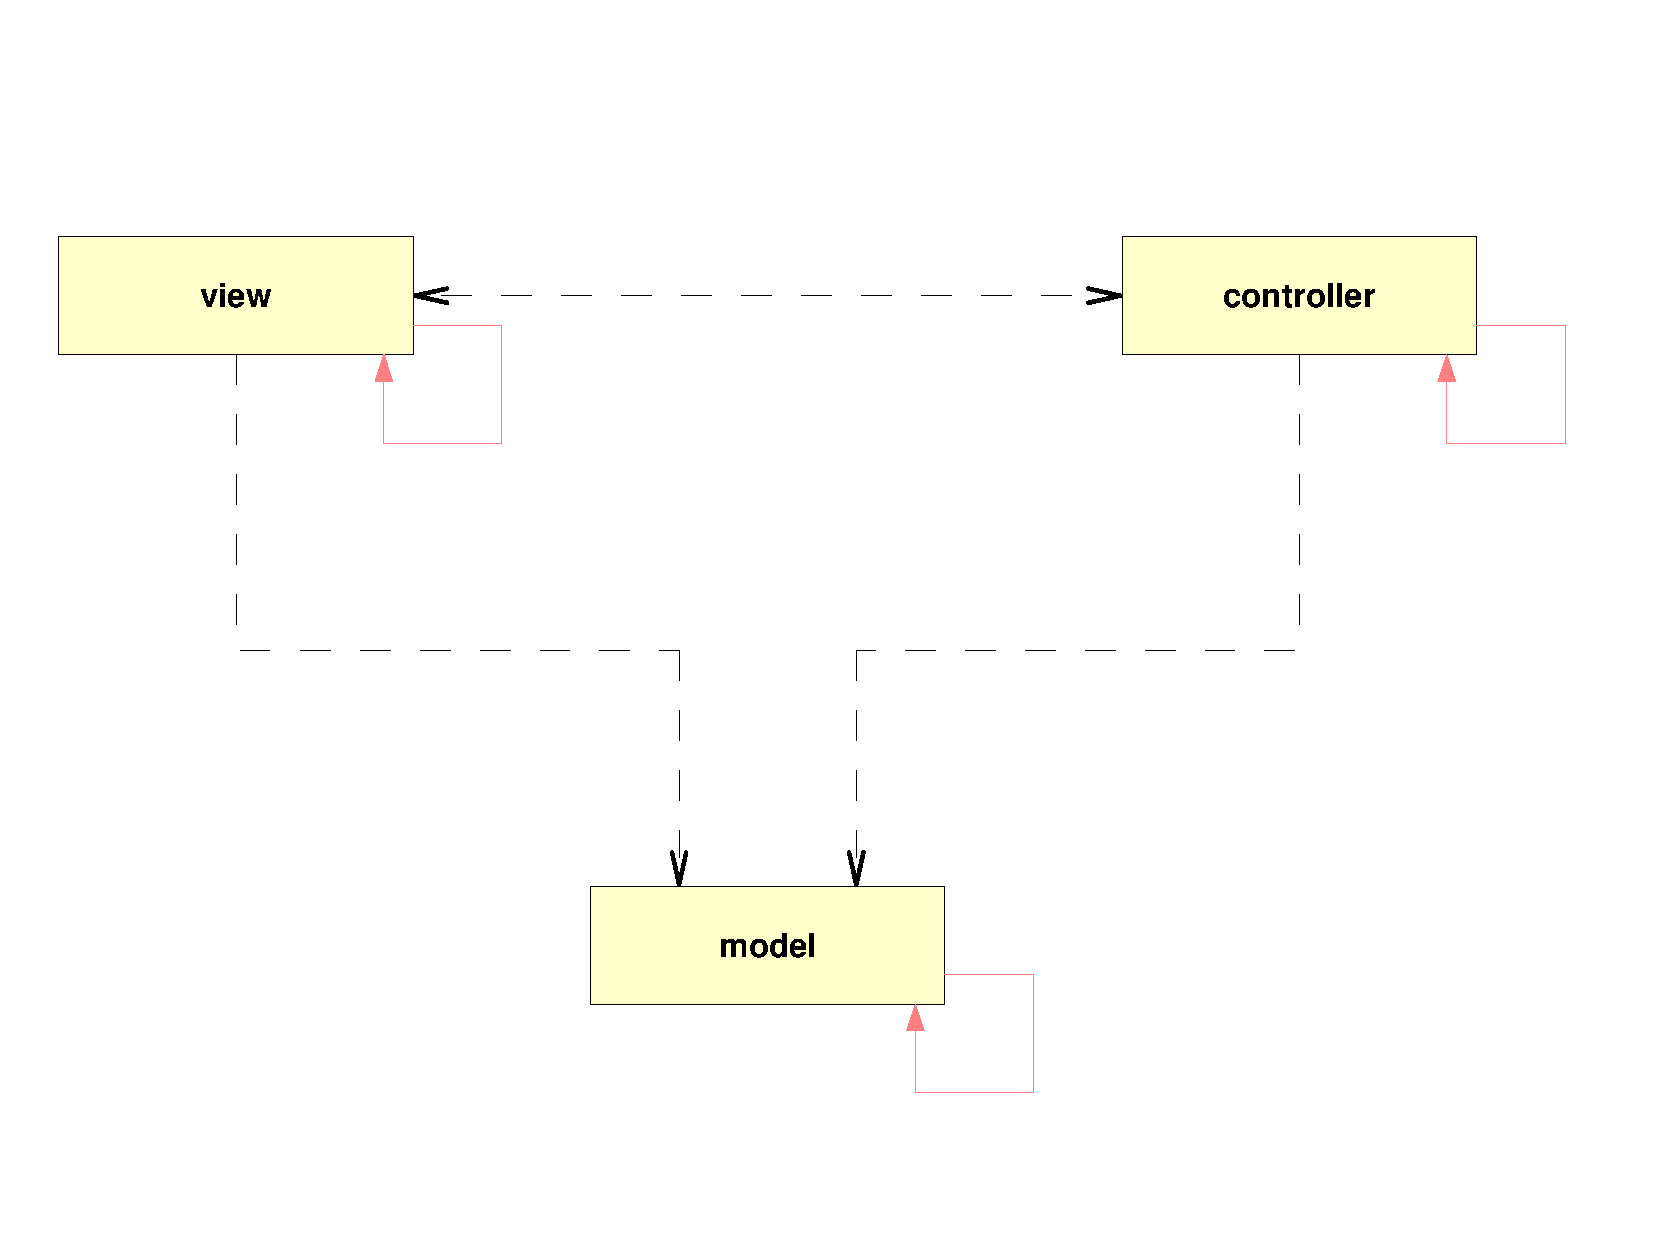
\includegraphics[scale=0.3,angle=-90]{graphic/adapted.pdf}
        \caption{Adapted (H)MVC Pattern with Hierarchical Elements}
        \label{adapted_figure}
    \end{center}
\end{figure}

The MVC pattern (figure \ref{adapted_figure}) consists of a \emph{View} that is
mostly implemented as \emph{Graphical User Interface} (GUI) frame with panel,
menubar, menu items and smaller components which, in this order, are all part
of the frame's hierarchy. Then, there is the \emph{Controller}. The
\emph{Hierarchical Model View Controller} (HMVC) pattern (section
\ref{hierarchical_model_view_controller_heading}) suggested to use a controller
hierarchy consisting of \emph{MVC Triads}. Finally, there is the \emph{Model}
of domain concepts which not only knowledge systems can structure
hierarchically. Reflecting these facts, one question is at hand:

\begin{quote}
    If View, Controller and Model ideally have a hierarchical structure,\\
    why not creating whole software systems after this paradigm?\\
    Isn't every system, in essence, just a \emph{Tree} of items?
\end{quote}
